\documentclass[tikz,border=6pt]{standalone}
\usepackage[T1]{fontenc}
\usepackage{helvet}
\renewcommand{\familydefault}{\sfdefault}
\usetikzlibrary{positioning,arrows.meta,calc,fit,shapes.geometric,shapes.misc,shapes.multipart}
\newcommand{\dt}{\,\textperiodcentered\,}
\tikzset{
  arr/.style={-{Latex[length=2.2mm]},line width=0.6pt},
  darr/.style={{Latex[length=2.2mm]}-{Latex[length=2.2mm]},line width=0.6pt},
  dashedarr/.style={-{Latex[length=2.2mm,open]},line width=0.6pt,dashed},
  retarr/.style={-{Latex[length=2.2mm]},line width=0.6pt,dashed},
  lbl/.style={font=\footnotesize\itshape},
}

% Sequence-diagram helpers: lifelines at fixed x, messages at a y row.
\newcommand{\lifeline}[4]{% name, x, label, bottom-y
  \node[draw,rounded corners=3pt,align=center,font=\small\bfseries,minimum width=2.9cm,minimum height=1.1cm,line width=0.7pt] (#1) at (#2,0) {#3};
  \draw[dashed,line width=0.5pt] (#2,-0.55) -- (#2,#4);}
\newcommand{\msg}[4]{% y, fromx, tox, text  (solid call)
  \draw[arr] (#2,#1) -- node[font=\footnotesize\bfseries,above,midway,align=center,fill=white,inner sep=1pt]{#4} (#3,#1);}
\newcommand{\ret}[4]{% y, fromx, tox, text  (dashed return)
  \draw[retarr] (#2,#1) -- node[font=\footnotesize,above,midway,align=center,fill=white,inner sep=1pt]{#4} (#3,#1);}
\newcommand{\selfmsg}[3]{% y, x, text
  \draw[arr] (#2,#1) -- ++(0.6,0) -- ++(0,-0.45) -- ++(-0.6,0);
  \node[font=\footnotesize\itshape,anchor=west,align=left,fill=white,inner sep=1.5pt] at (#2+0.75,#1-0.22) {#3};}
\newcommand{\altframe}[6]{% x0, y-top, x1, y-bottom, y-divider, guards {a}{b}
  \draw[line width=0.6pt] (#1,#2) rectangle (#3,#4);
  \draw[line width=0.6pt] (#1,#2) -- ++(1.0,0) -- ++(0,-0.42) -- ++(-0.25,-0.22) -- ++(-0.75,0);
  \node[font=\small\bfseries,anchor=north west] at (#1+0.12,#2-0.04) {alt};
  \draw[dashed,line width=0.5pt] (#1,#5) -- (#3,#5);
  \node[font=\footnotesize\itshape,anchor=west] at (#1+1.2,#2-0.3) {#6};}

\begin{document}
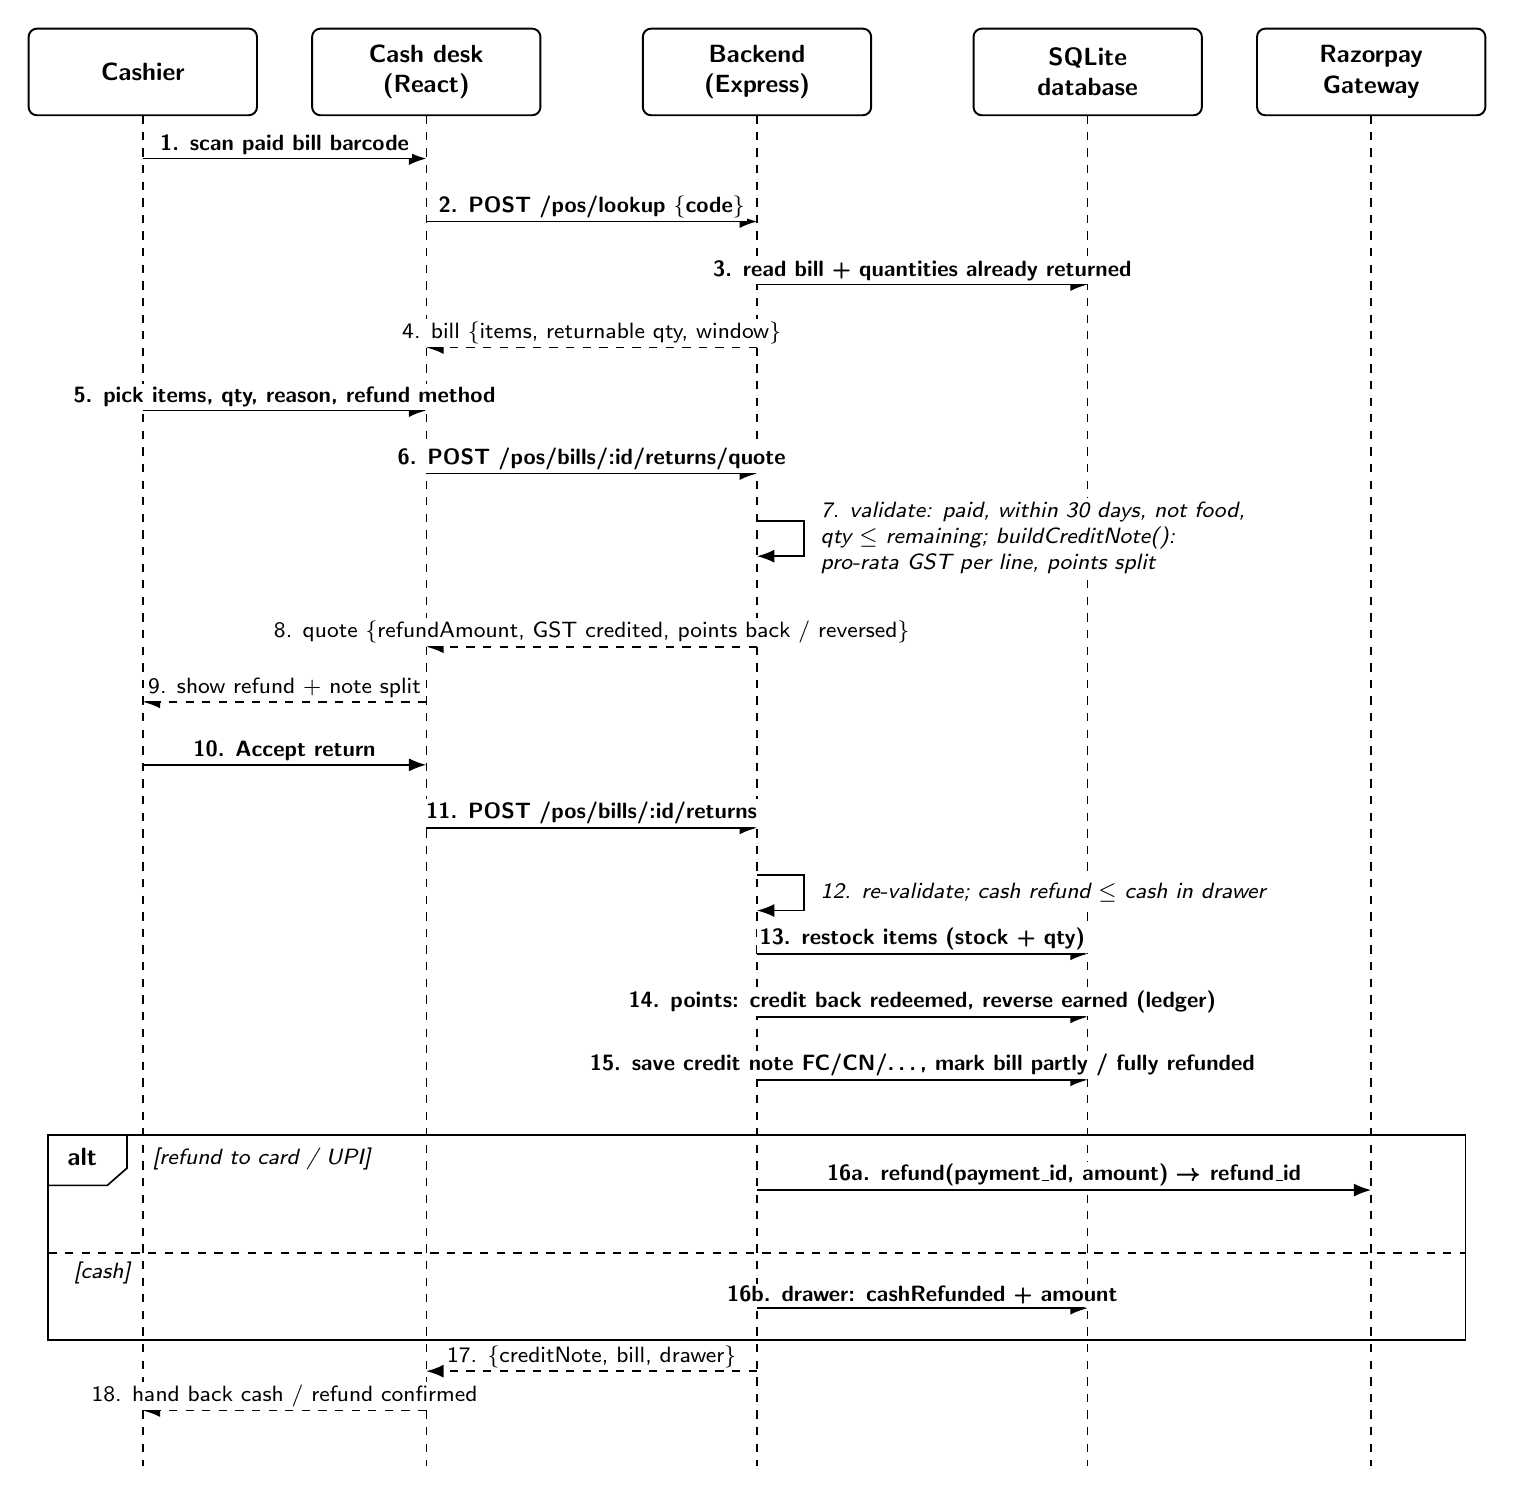
\begin{tikzpicture}
\def\C{0}\def\F{3.6}\def\B{7.8}\def\D{12.0}\def\R{15.6}
\lifeline{c}{\C}{Cashier}{-17.7}
\lifeline{f}{\F}{Cash desk\\(React)}{-17.7}
\lifeline{b}{\B}{Backend\\(Express)}{-17.7}
\lifeline{d}{\D}{SQLite\\database}{-17.7}
\lifeline{r}{\R}{Razorpay\\Gateway}{-17.7}
\msg{-1.1}{\C}{\F}{1. scan paid bill barcode}
\msg{-1.9}{\F}{\B}{2. POST /pos/lookup \{code\}}
\msg{-2.7}{\B}{\D}{3. read bill + quantities already returned}
\ret{-3.5}{\B}{\F}{4. bill \{items, returnable qty, window\}}
\msg{-4.3}{\C}{\F}{5. pick items, qty, reason, refund method}
\msg{-5.1}{\F}{\B}{6. POST /pos/bills/:id/returns/quote}
\selfmsg{-5.7}{\B}{7. validate: paid, within 30 days, not food,\\qty $\leq$ remaining; buildCreditNote():\\pro-rata GST per line, points split}
\ret{-7.3}{\B}{\F}{8. quote \{refundAmount, GST credited, points back / reversed\}}
\ret{-8.0}{\F}{\C}{9. show refund + note split}
\msg{-8.8}{\C}{\F}{10. Accept return}
\msg{-9.6}{\F}{\B}{11. POST /pos/bills/:id/returns}
\selfmsg{-10.2}{\B}{12. re-validate; cash refund $\leq$ cash in drawer}
\msg{-11.2}{\B}{\D}{13. restock items (stock + qty)}
\msg{-12.0}{\B}{\D}{14. points: credit back redeemed, reverse earned (ledger)}
\msg{-12.8}{\B}{\D}{15. save credit note FC/CN/\ldots, mark bill partly / fully refunded}
\altframe{-1.2}{-13.5}{16.8}{-16.1}{-15.0}{[refund to card / UPI]}
\msg{-14.2}{\B}{\R}{16a. refund(payment\_id, amount) \textrightarrow\ refund\_id};
\node[font=\footnotesize\itshape,anchor=west] at (-1.0,-15.25) {[cash]};
\msg{-15.7}{\B}{\D}{16b. drawer: cashRefunded + amount}
\ret{-16.5}{\B}{\F}{17. \{creditNote, bill, drawer\}}
\ret{-17.0}{\F}{\C}{18. hand back cash / refund confirmed}
\end{tikzpicture}
\end{document}
